\documentclass{article}
\usepackage[utf8]{inputenc}
\usepackage{geometry}
\usepackage{xcolor}
\usepackage{graphicx}
\usepackage{array}% figures in tables
\usepackage[export]{adjustbox} % crop graphics
\usepackage{amsmath}
\usepackage{amssymb}
\usepackage{amsfonts}
\usepackage{hyperref}
\usepackage{amsthm}
\usepackage{tikz}
\usepackage{stmaryrd} % pour les brackets
\usepackage{mathtools} % pour mathclap
\usepackage{soul} % \hl
%\usepackage{ulem}
\usepackage[english, onelanguage, ruled, lined, linesnumbered]{algorithm2e}
\usepackage{listings}
\usepackage[colorinlistoftodos]{todonotes}%TITLEPAGE
\usepackage{colortbl}
\usepackage{makecell}
\usepackage{pgf,tikz}
\usepackage{pstricks-add}
\usetikzlibrary{arrows,plotmarks,patterns,patterns.meta}

\title{MO-MILP Primal Heuristics\\ \large{Improvement of Gravity Machine}}
\author{Erwan Meunier}
\date{Computing Project, Nantes Université
\\ under the supervision of Xavier Gandibleux and Saïd Hanafi
\\ January - May 2023}
%Changer les marges

\def\noteXavier#1{\textcolor{olive}{\scriptsize [XG] #1}}
\def\noteSaid#1{\textcolor{red}{\scriptsize [SH] #1}}
\def\noteErwan#1{\marginpar{\textcolor{brown}{\scriptsize [EM] #1}}}

\newcommand{\set}[1]{\left\lbrace #1 \right\rbrace}

%\RestyleAlgo{ruled}

%% This is needed if you want to add comments in
%% your algorithm with \Comment
\SetKwComment{Comment}{/* }{ */}

\newtheorem{definition}{Definition}

\newtheorem{theorem}{Theorem}[section]

\newtheorem{corollary}{Corollary}[theorem]

\newtheorem{proposition}{Proposition}

\newtheorem{lemma}{Lemma}

\begin{document}
\begin{titlepage}

\newcommand{\HRule}{\rule{\linewidth}{0.5mm}} % Defines a new command for the horizontal lines, change thickness here

%----------------------------------------------------------------------------------------
%	LOGO SECTION
%----------------------------------------------------------------------------------------
\centering

\includegraphics[width=8cm]{logos/Logotype_Nantes-U_noir-300dpi.png}\\[1cm] % Include a department/university logo - this will require the graphicx package
 
%----------------------------------------------------------------------------------------

\center % Center everything on the page

%----------------------------------------------------------------------------------------
%	HEADING SECTIONS
%----------------------------------------------------------------------------------------

\textsc{\LARGE Computing Project \\ - \\ First year of Master's Degree in Optimization and Operations Research}\\[1.5cm] 
\textsc{\Large LS2N - Laboratory of Digital Sciences of Nantes}\\[0.5cm] 
\textsc{\large Team MODELIS - Modélisation Optimisation et DEcision pour la Logistique, l'Industrie et les Services}\\[0.5cm] 

%----------------------------------------------------------------------------------------
%	TITLE SECTION
%----------------------------------------------------------------------------------------
\makeatletter
\HRule \\[0.4cm]
{ \huge \bfseries \@title}\\[0.4cm] % Title of your document
\HRule \\[1.5cm]
 
%----------------------------------------------------------------------------------------
%	AUTHOR SECTION
%----------------------------------------------------------------------------------------

\begin{minipage}{0.4\textwidth}
\begin{flushleft} \large
\emph{Author:}\\
\@author$^1$ % Your name

\end{flushleft}
\end{minipage}
~
\begin{minipage}{0.4\textwidth}
\begin{flushright} \large
\emph{Under the direction of:} \\
Xavier Gandibleux$^2$ \\
Saïd Hanafi$^3$\\[1.2em]
\end{flushright}
\end{minipage}\\[2cm]
\let\thefootnote\relax\footnote{$^1$\texttt{erwan.meunier@etu.univ-nantes.fr}}
\let\thefootnote\relax\footnote{$^2$\texttt{xavier.gandibleux@univ-nantes.fr}}
\let\thefootnote\relax\footnote{$^3$\texttt{said.hanafi@uphf.fr}}
\makeatother

%----------------------------------------------------------------------------------------
%	DATE SECTION
%----------------------------------------------------------------------------------------

{\large Defended on \today}\\[2cm] % Date, change the \today to a set date if you want to be precise

\vfill % Fill the rest of the page with whitespace

\end{titlepage}
%\maketitle
\newpage
\tableofcontents
\newpage
\section{Abstract}

\newpage
\section{Introduction}


\newpage
\section{Definitions and Notations}
We consider the problem as presented in \cite{gravitymachine}. The multi-objective 0-1 linear optimisation problems with $p$ objectives ($p$-01LP) considered can be formulated as follows:
\begin{align*}
    \min z(x)&=Cx\\
    \text{subject to } Ax &\leqq b\\
    x &\in \set{0,1}^n
\end{align*}
where
\begin{itemize}
    \item $x\in \set{0,1}^n$, the vector of $n$ binary variables $x_j, j=1,\ldots,n$;
    \item $A\in\mathbb{R}^{m\times n}$, the $m$ constraints $A_ix \leq b_i, \; i=1,\ldots,m$ and $b\in \mathbb{R}^m$;
    \item $C \in \mathbb{R}^{p\times n}$, the objective matrix where $p \geq 2$;
    \item $X:=\set{x\in\set{0,1}^n\mid Ax \leqq b} \subseteq \mathbb{R}^n$, the set of feasible solutions, with $\mathbb{R}^n$ the decision space;
    \item $Y:=\set{Cx\mid x \in X}\subseteq\mathbb{R}^p$, the outcome set, with $\mathbb{R}^p$ the objective space.
\end{itemize}
Thereafter, $p$ is usually meant to be equal to $2$ (\textit{e.g.} we consider the bi-objective class of problems).
\begin{definition}[\cite{MultOptEhrgott}]
A feasible solution $\hat{x}\in\mathcal{X}$ is called efficient or Pareto optimal if there is no other $x \in \mathcal{X}$ such that $f(x)\leq f(\hat{x})$. If $\hat{x}$ is efficient, $f(\hat{x})$ is called nondominated point. If $x^1, x^2 \in \mathcal{X}$ and $f(x^1)\leq f(x^2)$ we say $x^1$ dominates $x^2$ and $f(x^1)$ dominates $f(x^2)$. The set of all efficient solutions $\hat{x} \in \mathcal{X}$ is denoted $\mathcal{X}_E$ and called the efficient set. The set of all nondominated points $\hat{y}=f(\hat{x})\in\mathcal{Y}$, where $\hat{x}\in\mathcal{X}_E$, is denoted $\mathcal{Y}_N$ and called the nondominated set.
\end{definition}
\begin{definition}[\cite{MultOptEhrgott}]
A feasible solution $\hat{x}\in \mathcal{X}$ is called weakly efficient (weakly Pareto optimal) if there is no $x\in \mathcal{X}$ such that $f(x)<f(\hat{x})$, \textit{i.e.} $f_k(x)<f_k(\hat{x})$ for all $k=1,\ldots,p$. The point $\hat{y}=f(\hat{x})$ is then called weakly nondominated. A feasible solution $\hat{x}\in\mathcal{X}$ is called strictly efficient (strictly Pareto optimal) if there is no $x\in\mathcal{X}$,$x\neq\hat{x}$ such that $f(x)\leqq f(\hat{x})$. The weakly (strictly) efficient and nondominated sets are denoted $\mathcal{X}_{wE}(\mathcal{X}_{sE})$ and $ \mathcal{Y}_{wE}$, respectively. 
\end{definition}

\begin{definition}[A lower bound set~\cite{boundssetsXGME}]
A lower bound set for $Y'$ is a subset $L \subseteq \mathbb{R}^p$
\begin{enumerate}
    \item For each $y\in Y'$ there is some $l\in L$ such that $l\leqq y$
    \item There is no pair $y\in Y',l\in L$ such that $y$ dominates $l$.
\end{enumerate}
\end{definition}
\begin{definition}[An upper bound set~\cite{boundssetsXGME}]
An upper bound set for $Y'$ is a subset $U \subset \mathbb{R}^p$
\begin{enumerate}
    \item For each $y\in Y'$ there is some $u\in U$ such that $y\leqq u$
    \item There is no pair $y\in Y',\in U$ such that $u$ dominates $y$.
\end{enumerate}
\end{definition}
%\pagestyle{empty}
\definecolor{ttfftt}{rgb}{0.2,1,0.2}
\definecolor{ffwwww}{rgb}{1,0.4,0.4}
\definecolor{qqttff}{rgb}{0,0.2,1}
\definecolor{qqqqff}{rgb}{0,0,1}
\definecolor{ttttff}{rgb}{0.2,0.2,1}
\definecolor{fftttt}{rgb}{1,0.2,0.2}
\definecolor{cqcqcq}{rgb}{0.75,0.75,0.75}
\begin{tikzpicture}[line cap=round,line join=round,>=triangle 45,x=10.0cm,y=10.0cm]
\draw [color=cqcqcq,dash pattern=on 2pt off 2pt, xstep=2.0cm,ystep=2.0cm] (-0.4,-0.2) grid (1.4,1.2);
\draw[->,color=black] (-0.4,0) -- (1.4,0);
\foreach \x in {-0.4,-0.2,0.2,0.4,0.6,0.8,1,1.2,1.4}
\draw[shift={(\x,0)},color=black] (0pt,2pt) -- (0pt,-2pt) node[below] {\footnotesize $\x$};
\draw[->,color=black] (0,-0.2) -- (0,1.2);
\foreach \y in {-0.2,0.2,0.4,0.6,0.8,1}
\draw[shift={(0,\y)},color=black] (2pt,0pt) -- (-2pt,0pt) node[left] {\footnotesize $\y$};
\draw[color=black] (0pt,-10pt) node[right] {\footnotesize $0$};
\clip(-0.4,-0.2) rectangle (1.4,1.2);
\fill[color=ttfftt,fill=ttfftt,fill opacity=0.1] (0,1) -- (1,1) -- (1,0) -- cycle;
\draw [line width=1.6pt,dash pattern=on 3pt off 3pt,color=ffwwww,domain=-0.4:1.4] plot(\x,{(--1-1*\x)/1});
\draw [color=ttfftt] (0,1)-- (1,1);
\draw [color=ttfftt] (1,1)-- (1,0);
\draw [color=ttfftt] (1,0)-- (0,1);
\begin{scriptsize}
\fill [color=fftttt] (0,0) circle (2.5pt);
\draw[color=fftttt] (0.05,0.04) node {$(0, 0)$};
\fill [color=ttttff] (0,1) circle (2.5pt);
\draw[color=ttttff] (0.05,1.04) node {$(0, 1)$};
\fill [color=qqqqff] (1,1) circle (2.5pt);
\draw[color=qqqqff] (1.05,1.04) node {$(1, 1)$};
\fill [color=qqttff] (1,0) circle (2.5pt);
\draw[color=qqttff] (1.05,0.04) node {$(1, 0)$};
\draw[color=ffwwww] (-0.59,1.67) node {$x + y = 1$};
\end{scriptsize}
\end{tikzpicture}

\begin{figure}
    \centering
    \includegraphics[scale=0.45]{figures_tikz/figure1_exempleCOST.png}
    \caption{Projection of the solution space onto the cost space}
    \label{fi:costspace}
\end{figure}

\section{Gravity Machine}
Gravity Machine is an algorithm aiming to compute an upperbound set for a multi-objective linear optimization problem with binary variables.
It is based the on the \textit{Feasibilty Pump} \cite{FeasibilityPump} which is a heuristic for finding a feasible solution of a given MIP.
The essence of this well studied heuristic \cite{ten_years_fp} is given by:

\begin{algorithm}[h!]
    \caption{Feasibilty Pump (basic version)}
    \KwData{$\text{termination\_criteria}$, $T\in\mathbb{N}^*$}
    \KwResult{A feasible solution or nothing}
    \Begin{
        $nIT \gets 0$\;
        $x^* \gets \text{argmin} \set{c^Tx:Ax\geq b}$\;
        \eIf{$x^* \text{is integer}$}{\Return{$x^*$}}{
            $\Tilde{x} \gets \left[x^*\right]$\;
            \While{$\neg \text{termination\_criteria}$}{
                $nIT \gets nIT + 1$\;
                $x^* \gets \text{argmin} \set{\Delta(x,\Tilde{x}):Ax\geq b}$\;
                \uIf{$x^* \text{is integer}$}{
                    \Return{$x^*$}\;
                }\uElseIf{$\exists j \in \mathcal{I}:\left[x_j^*\right]\neq \Tilde{x}_j$}{
                    $\Tilde{x} \gets \left[x^*\right]$
                }
                \Else{
                    $\mathcal{X} \gets \textsc{sort}\left(\mathcal{I},\text{by highest} \left| x_j^* - \Tilde{x}_j \right| \right)$\;
                    $k \gets \textsc{rand}\left(\frac{T}{2},\frac{3T}{2}\right)$\;
                    $\textsc{flip} \text{ the } k \text{ first entries } \Tilde{x}_j \in \mathcal{X}$\; 
                }
            }
        }
    }
\end{algorithm}

\subsection{Generators}
\subsection{Projection}
\subsection{Rounding}
\subsection{Perturbing}

\begin{algorithm}[h!]
    \caption{Outline of Gravity Machine}\label{alg:Gravity_Machine_Initial}
    \KwData{$\mathcal{D}$,$n_L$,maxTrial,maxTime}
    \KwResult{$L$,$U$}
    \Begin{
     $L,F \gets \textsc{ComputeGenerators}(\mathcal{D},n_L)$\;
     \ForAll(//each $k$-th unfeasible gen){$z(\bar{x}^k)\in L,\Bar{x}^k\notin F$}{
      timeStart $\gets \textsc{Time}()$; trial $\gets 0$\;
      timeout $\gets$ false; feasible $\gets$ false\;
      $\Tilde{x},H,cycle \gets \textsc{RoundingSolution}(\bar{x}^k,H)$\;
      \While{$\neg feasible \land \neg timeout$}{
       trial $\gets$ trial $+1$\;
       $\Bar{x},F$,feasible $\gets \textsc{ProjectSolution}(\Tilde{x})$\;
       \If{$\neg feasible$}{
            $\Tilde{x},H,cycle \gets \textsc{RoundingSolution}(\Bar{x},k,h)$\;
            \If{cycle}{
                $\Tilde{x}\gets\textsc{PerturbSolution}(\Tilde{x})$\;
            }
        }
        timeout $\gets$ (time()-timeStart $\geq$ maxTime) $\lor$ (trial=maxTrial)\;
       }
     }
     $U \gets \textsc{ExtractNonDominatedPoint}(F)$\;
     }
\end{algorithm}
    

\section{Improving generators}
Generators are obtained by using the $\epsilon$-constraints method which is one of the well-known scalarization techniques \cite{Chankong1983MultiobjectiveDM} aimed at getting a sample of efficient solutions of a MOLP. Those generators form an efficient set for the relaxed problem. That is to say, the set of all generators is also the lower bound set $L$. Since GM starts the search based on each $k$-th generator, one would like to have a better initial solution in order to reach a feasible solution faster.

\subsection{Bugs in Gravity Machine}

\subsubsection{Generators not feasible}
The previous version of Gravity Machine did use the GLPK solver to generate the lower bound set by the $\epsilon$-constraints method. 
However, closer to the line passing through the Nadir and the origin the more constrained the MILP representing the current generator. 
Since considered problems have lot of constraints and variables some numerical issues may arise \cite{gurobiNumIssues}. Infeasibility hence
may appear during the solving process for problems which has at least one (feasible) optimal solution. In addition, the \textit{Julia} wrapper
for GLPK seems to be known for returning the solution minimizing constraints violation\footnote{\url{https://discourse.julialang.org/t/access-infeasible-optimization-results-glpk-with-semicontinuous-variable/59972}}.
Finally, as the termination status was not correctly handled, some generators turn out to be used whereas there were not "trully" feasible.
\paragraph*{Patch:}
The termination status is now considered and GM properly fails if a generator is not feasible. 
Tolerance attribute was hand-tuned to allow the solver to find a feasible solution. \noteErwan{ça serait bien que ce ne soit pas "hand-tuned" \url{}https://discourse.julialang.org/t/scalling-both-primal-and-dual-feasibility-tolerance-according-to-the-size-of-the-problem/97455}.
It is worth noticing that no difference in the performance has been observed. The robustness is the matter here.
In addition, GLPK was replaced by HiGHS~\cite{highs}. Indeed, the latter shows better performances than GLPK~\cite{bench_solver} and is still open-source.

\subsubsection{Soft conic constraints $\lambda_1$ and $\lambda_2$}
Both vectors $\lambda_1$ and $\lambda_2$ were accidentaly swaped in their definition such that the "guidance mechanism" was useless and a fortiori misleading.

\subsection{Empirical findings}
Empirical evidences tend to show that very few variables are set to non-integral value for each generator.
%TODO

\subsection{Setting some variables binary}
At first sight, non-solved to integrality variables should be set binary and the problem re-optimized. The latter allows GM to find initial solution Then, a generator closer to $Y$ should result from a the re-optimization process. However, several issues arises:

\subsubsection{Communicating vessels effect}
Since not all constraints are set binary, some variables found to be zero or one might become fractional. 
A number of variables found fractional after the second stage solving greater than the number of variables found fractional after the first stage solving represents the worst case. 
As far as our experimental results show us, this situation is very rare. \noteErwan{à reformuler}
%TODO
\subsubsection{Same generators lead to the same solution}
Ideally, one would that each generator $\bar{y}^k$ converges to a different $\Tilde{y}^{k,t}$ for some iterations $t\in \mathbb{N}$.
Below, we consider $J_0(x)$ (and $J_1(x)$) the set containing the index of variables set to zero (respectively to one) into the solution $x$.
Some well known modelization techniques are briefly presented and their pertinence for GM is studied. For the major part of them, 
they are inspired by canonical cut constraints introduced by~\cite{canonical_cut} and used for the same purpose by~\cite{Hanafi2011}.

\paragraph*{Canonical cut constraint:}
\begin{proposition}\label{bincutconstraintexact}
    Let $x^0$ be a vector in $\set{0,1}^n$. The following inequality
    \begin{equation}
        \sum_{j\in J_1(x^0)} x_j + \sum_{j \in J_1(x^0)} 1-x_ j \geq 1
    \end{equation}
    cutts off solution $x^0$ without cutting off any other solution in $\set{0,1}^n$.
\end{proposition}
\begin{proof}
Let's suppose that $x^0$ is not cutted off by the constraint. Then $x = x^0$ implies $0\geq 1$ from (1). The cutting off is proved.
\\Finally, a solution $x^1 \neq_1 x^0$ is assumed to be cutted off by the constraint. That is to say
\begin{align}
    & \sum_{j\in J_1(x^0)} x_j^1 + \sum_{j \in J_1(x^0)} 1-x_ j^1 = 0 \\
    \Longleftrightarrow &   \| x^0 - x^1 \| = 0
\end{align}
In other words $x^0 = x^1$ and $x^0 \neq x^1$ which is impossible. Then,~\ref{bincutconstraintexact} holds.
\end{proof}
\begin{proposition}
    Gravity Machine does not longer guarantee the rectitude of $L$ if $x^0\in \left\lbrack 0,1 \right\rbrack ^n$
\end{proposition}
\begin{proof}
    We exhibit a counter-example. Let be a $1$-01LP of the form:
    \begin{align}
        \text{Min}  & \quad x_1 + x_2\\
        s.t & \quad x_1 + x_ 2 \geq \frac{1}{4}\\
        & -x_1 + x_2 \geq -\frac{3}{4}\\
        & x_1, \: x_2 \in \set{0,1}
    \end{align} 
    According to~\ref{fig:counterExampleL}, $x^* = \left(0,1\right)$ is clearly the optimal solution whereas 
    the optimal solution for the relaxed problem is $x^0 = \left( 0, \frac{1}{4}\right)$.
    Since, $x_1$ has a continuous value, only $x_2$ is present in the new constraint:
    \begin{equation}
        1-x_2 \geq 1 \Leftrightarrow x_2 = 0
    \end{equation}
    Consequently, this new constraint prevent the solver finding the $x^*$ and what is more make the problem infeasible.
\end{proof}
\begin{figure}
    \centering
    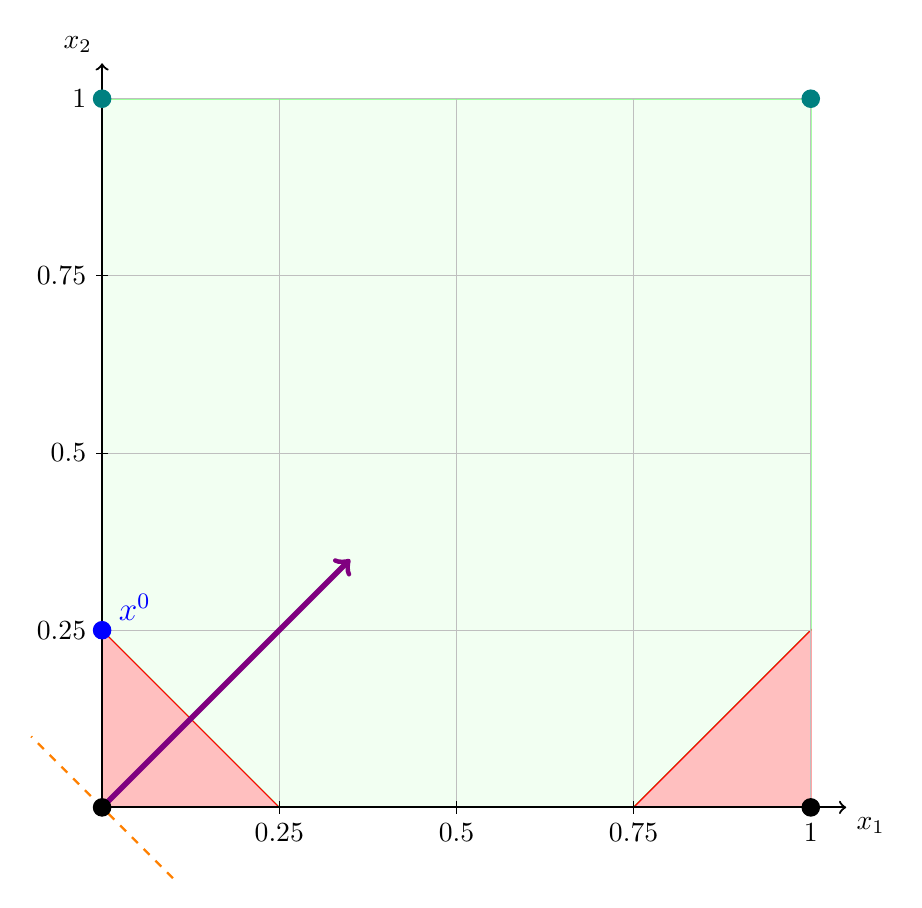
\begin{tikzpicture}[scale=9]
        \filldraw[fill=green!5,draw=green] (0,0.25)--(0,1)--(1,1)--(1,0.25)--(0.75,0)--(0.25,0)--cycle;
        \filldraw[fill=red!25,draw=red] (0,0)--(0,0.25)--(0.25,0)--cycle;
        \filldraw[fill=red!25,draw=red] (1,0)--(1,0.25)--(0.75,0)--cycle;
        \draw[step=0.25cm,color=gray!50] (0,0) grid (1,1);
        \foreach \x in {0.25,0.5,0.75,1}{
            \draw (\x cm, 0.25pt) -- (\x cm,-0.25pt) node[anchor=north] {$\x$};
        }
        \foreach \y in {0.25,0.5,0.75,1}{
            \draw (0.25pt, \y cm) -- (-0.25pt,\y cm) node[anchor=east] {$\y$};
        }
        \draw[thick,->] (0,0)--(1.05,0) node[anchor=north west] {$x_1$};
        \draw[thick,->] (0,0)--(0,1.05) node[anchor=south east] {$x_2$};
        \draw[->,violet,line width=2pt] (0,0)--(0.35,0.35);
        \draw[orange, dashed,thick] (0.1,-0.1)--(-0.1,0.1);
        \foreach \x/\y in {0/0, 1/0}{
            \filldraw[black] (\x,\y) circle (0.35pt);
        }
        \foreach \x/\y in {0/1, 1/1}{
            \filldraw[teal] (\x,\y) circle (0.35pt);
        }
        \filldraw[blue] (0,0.25) circle (0.35pt);
        \node[above right,blue] at (0.01,0.25) {\large \textbf{$x^0$}};
    \end{tikzpicture}
    \caption{Illustration of the counter-example}\label{fig:counterExampleL}
\end{figure}
\paragraph{Cones}

\begin{algorithm}
\caption{Improving generators}\label{alg:Generators_improvement}
\KwData{$L$,$\lambda_1$,$\lambda_2$,$\tau$,$\alpha$}
\KwResult{$L_I$,$U$}
\Begin{
 $L,F \gets \textsc{ComputeGenerators}(\mathcal{D},n_L)$\;
 \ForAll(//each $k$-th unfeasible gen){$z(\bar{x}^k)\in L,\Bar{x}^k\notin F$}{
  
 }
 }
\end{algorithm}
\subsubsection{Too much binary variables increase the solving time}
As shown by our empirical data, less than 20

\section{Improving projection}
By the same token as the generators improvement, the projection used during GM can be improved by adding some integrity constraints on the non 



\section{Numerical experiments}
Gravity Machine is implemented in Julia 1.8.5 \cite{Julia-2017}
\subsection{Numerical instances}
\subsection{Quality measure}
\subsection{Numerical results}
Experiments have been performed on-top of the following configuration:
\begin{itemize}
    \item Laptop: Dell - XPS 13 9300
    \item OS: Linux Mint 21.1 Cinnamon - v5.6.8
    \item Kernel version: 5.19.0-38-generic
    \item Intel© Core™ i7-1065G7 CPU @ 1.30GHz × 4
    \item L1: 320 KiB, L2: 2 MiB, L3: 8 MiB
    \item RAM: 15.2 Go LDDR4
    \item SSD: 1024.2 Go
\end{itemize}



\input{code}

\section{Conclusion and discussion}
%\section{Questionnements et idées}
Légende : \hl{$\Box$} signifie "point important"
Pour le 17/01
\begin{itemize}
    \item \hl{$\Box$} \textsc{PerturbSolution} $\leadsto$ Mesurer l'impact de $T$ sur FP ?
    \begin{itemize}
        \item Cela a-t-il déjà été mesuré dans le cas mono-objectif ?
        \item Peut-on transférer de potentielles conclusions du mono sur du multi ?
        \item Possibilité de faire bouger $T$ en fonction de l'avancement dans l'algorithme ? Comment ? $\leadsto$ Patch pour diminuer le cyclage ?
    \end{itemize}
    \item \hl{$\Box$} Mesurer l'impact de \texttt{tailleSampling} sur le ration $\frac{quality}{time}$
    \item Seuil de tolérance dans \textsc{roundingSolution} $\leadsto$ atol=$10^{-3}$ pas un peu trop grand ? Standard ?
    \item \hl{$\Box$} Utiliser l'amélioration de FP proposée par~\cite{improvedFP}
    \item Point de détail pas important : \textsc{elaborePointConeOuvertversL} considère les points dans l'ordre inverse de la convention graphique adoptée dans l'article \textit{i.e.} les $y_k$ ne "descendent pas au fur et à mesure que $k$ est grand" mais l'inverse. 
    \item Mesurer en quel proportion $p_N$ domine $p_C$ dans la conditionnelle de \textsc{elaborePointConeOuvertversL} $\leadsto$ pour quel(s) impact(s) ?
    \item L'article affirme que \textsc{GravityMachine} n'est pas problème dépendant, cependant son efficacité est seulement mesurée sur le SPA qui a par hypothèse une structure particulière ?
    \item $\leadsto$ Générer des instances aléatoirement sans structure autres que les contraintes d'intégrités et benchmarker en fonction des caractéristiques de chaque instance : nombre de contraintes, contraintes très "couvrantes", nombre de variables, etc $\leadsto$ Existe-t-il des mesures pertinentes des caractéristiques d'une instance ?
    \item ??? Fractions pour $\lambda_1$ et $\lambda_2$ dans \textsc{calculerDirections2} peuvent-être simplifiées en $\frac{\Delta y}{\Delta x + \delta y}$ et $\frac{\Delta x}{\Delta x + \Delta y}$. En regardant le \textsc{$\Delta$SPA2bis} et \textsc{calculerDirections2} j'ai les intuitions suivantes :
    \begin{itemize}
        \item Plus $\Delta y$ est grand plus 
    \end{itemize}
\end{itemize}
Pour le 24/01
\begin{itemize}
    \item Tester les composants de manière indépendante : \url{https://uditagarwal.in/understanding-dependency-graphs-for-program-analysis/}
    \item Analyser les points qui voient le moins de contraintes
    \item Utiliser le centre analytique pour guider les arrondis
\end{itemize}
Pour le 31/01
\begin{itemize}
    \item Densifier  les générateurs quand on se rapproche de la droite $z^2(x)=z^1(x)$
    \item Restreindre la recherche par cône en utilisant le point idéal
    \item 
\end{itemize}
\section{Objectifs}
Pour la séance du 24/01
\begin{itemize}
    \item Choix de la projection
    \begin{itemize}
        \item Autres normes
        \item Actions sur $\lambda$ 
        \begin{itemize}
            \item Faire varier le $\lambda$ entre bornes $\leadsto$ alterner phases d'intensifications et de diversifications
            \item Pondérer l'importance des objectifs avec $\lambda_{a,b} = a\lambda_1 c_1  + b\lambda_2 c_2$
        \end{itemize}
        \item Taille du sampling $\leadsto$ en déduire une borne sur les secteurs angulaires des cônes
        \item Calculer l'admissibilité de points entiers dans le cône puis tracer une famille de $\lambda_h$ selon quelques solutions entières admissibles.
    \end{itemize}
    \item Fixer $T$ convenablement en fonction de la taille du problème / valuation dynamique de $T$
\end{itemize}
Pour la séance du 09/02
\begin{itemize}
    \item 
\end{itemize}
Discussion annexes :
\begin{itemize}
    \item Validation de la pertinence de chaque version de chaque fonctionnalité et les interactions entre elles  $\leadsto$~\cite{irace}
    \item Générateurs d'instances 01 MO $\leadsto$ Voir mail de Xavier
\end{itemize}



\newpage
\bibliographystyle{apalike}
\bibliography{biblio.bib}
  
\section{Annexe}
\begin{table}[!ht]
    \centering
    \begin{tabular}{|c|c|c|c|}
        \hline
        Instance & Time & Quality &  \makecell{Number of supported\\ points found} \\ 
        \hline
        1 & 416.393 & 84.42 & 5 \\ 
        3 & 249.077 & 87.3 & 5 \\
        \rowcolor{gray!25} 
        4 & Time out & X & X \\ 
        6 & 23.874 & 92.56 & 5 \\ 
        7 & 22.625 & 86.69 & 4 \\ 
        8 & 0.452 & 88.55 & 3 \\ 
        9 & 8.225 & 85.52 & 5 \\ 
        10 & 0.647 & 86.27 & 2 \\ 
        11 & 11.838 & 95.09 & 3 \\ 
        12 & 0.208 & 90.62 & 5 \\ 
        13 & 42.496 & 89.26 & 5 \\ 
        14 & 622.631 & 73.35 & 4 \\ 
        15 & 0.319 & 100 & 2 \\ 
        \rowcolor{gray!25} 16 & Time out & X & X \\ 
        17 & 599.07 & 51.51 & 3 \\ 
        18 & 46.637 & 84.56 & 2 \\ 
        19 & 3.779 & 91.72 & 4 \\ 
        20 & 1.182 & 92.68 & 3 \\ 
        21 & 0.821 & 95.45 & 4 \\ 
        22 & 1.337 & 93.49 & 5 \\ 
        23 & 0.47 & 91.43 & 2 \\ 
        24 & 2.666 & 96.13 & 4 \\ 
        25 & 2.266 & 91.12 & 5 \\ 
        26 & 0.894 & 93.41 & 4 \\ 
        27 & 1.658 & 91.15 & 2 \\ 
        28 & 1.943 & 92.4 & 3 \\ 
        29 & 6.527 & 88.21 & 4 \\ 
        30 & 6.254 & 97.06 & 4 \\ 
        31 & 13.176 & 92.66 & 5 \\ 
        32 & 0.12 & 96.99 & 3 \\ 
        33 & 14.603 & 94.62 & 4 \\ 
        34 & 2.143 & 92.29 & 4 \\ 
        35 & 4.992 & 93.43 & 4 \\ 
        36 & 5.125 & 91.59 & 3 \\ 
        37 & 1.644 & 94.88 & 4 \\ 
        38 & 2.685 & 92.43 & 4 \\ 
        39 & 1.618 & 98.16 & 5 \\ 
        40 & 0.426 & 86.44 & 4 \\ 
        41 & 0.125 & 86.77 & 5 \\ 
        42 & 1.895 & 97.69 & 3 \\ 
        43 & 6.023 & 93.31 & 4 \\ 
        \hline
    \end{tabular}
    \caption{Instances solved exactly with 6 solutions at most}\label{tab:solveExactly}
\end{table}

\end{document}
